
\documentclass{pdfBooklets}
\usepackage[printwatermark]{xwatermark}
\usepackage{tikz}



\title{Warsztat Elektroniczny}
\author{%
	Projekt ,,Matematyka dla Ciekawych Świata'',\\
	Krzysztof Lasocki\\\normalsize\ttfamily <krz.lasocki@gmail.com>
}
\date  {2020-04-04}

\makeatletter\hypersetup{
	pdftitle = {\@title}, pdfauthor = {\@author}
}\makeatother


\begin{document}

\maketitle

\newwatermark[allpages,color=red!50,angle=45,scale=3,xpos=0,ypos=0]{Wersja robocza}

\textit{o czym to w ogole jest? napisac slowo wstepne. Uoporządkować rozdziały}

\section{Przetwornica zasilająca}

\textit{tbd}

\section{Obsługa multimetru}

Multimetr to przyrząd pomiarowy który posiada wiele funkcji. Najczęściej są to woltomierz (do pomiaru napięcia), amperomierz
(do pomiaru natężenia, potocznie zwanego prądem) oraz omomierz (do pomiaru rezystancji). Często spotyka się także funkcje:
\begin{itemize}
\item \emph{Test połączeń} (\textit{continuity mode}), oznaczany symbolem fali dźwiękowej (lub nuty), służy do sprawdzania połączeń elektrycznych.
  Miernik wydaje dźwięk jeśli między przewodami jest połączenie.
\item \emph{Pomiar diód} (\textit{diode check}), oznaczony symbolem diody, służy to sprawdzania diód i innych elementów półprzewodnikowych.
  Wyświetla spadek napięcia na testowanym złączu półprzewodnikowym.
\item \emph{Test tranzystorów} (pomiar h\textsubscript{FE}), służący do pomiaru wzmocnienia tranzystora. Najczęściej posiada oddzielne gniazdo
  na mierniku.
\item \emph{Pomiar pojemności}, służy do pomiarów kondensatorów
\item \emph{Pomiar temperatury}, najczęściej za pomocą termopary (dołączana do miernika).
\end{itemize}

Multimetr zachowuje się tak jak przyrząd pomiarowy którego funkcjonalność jest aktualnie wybrana. Oznacza to że należy go podłączać
tak samo, jak odpowiednie przyrządy pomiarowe. 

\subsection{Połączenie miernika}
W zależności od modelu, multimetr może posiadać od dwóch do czterech gniazd na przewody. Są to:
\begin{itemize}
\item Masa, oznaczana \textbf{COM} (od słowa \textit{common}). Tutaj podłącza się czarny przewód
\item Wejście pomiarowe dla woltomierza, ozn. symbolem \textbf{V}. Często także jest to wejście omomierza, oznaczone \textbf{$\Omega$},
  oraz testu diód (ozn. symbolem diody)
\item Wejście miliamperomierza, oznaczone symbolem \textbf{mA}. Jeżeli Twój miernik posiada trzy wejścia, to najczęściej jest ono
  tym samym wejściem, co poprzednie.
\item Wejście amperomierza, oznaczone symbolem \textbf{A}. Najczęściej również jest obok niego podany maksymalny dopuszczalny prąd
  oraz czas pomiaru
\end{itemize}
\begin{center}
  {\noindent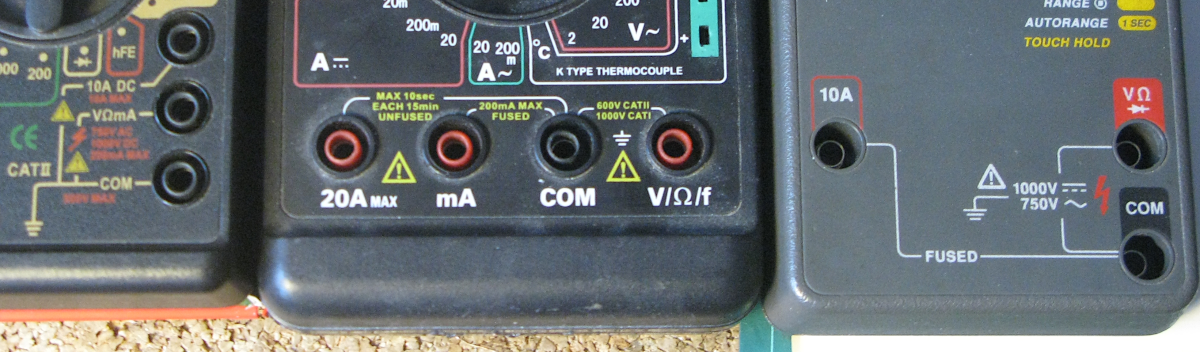
\includegraphics[width=0.9\textwidth,clip=true]{dmm_terminals.png}}\\
  Wejścia trzech różnych multimetrów. Pomiędzy wejściami zaznaczone są maksymalne wartości napięcia lub natężenia i informacja o zabezpieczeniach
  (``FUSED'') bądź ich braku (``UNFUSED'').\\
  Od lewej: typowy model z trzema wejściami, model z czterema wejściami, model z trzema wejściami (bez miliamperomierza)
\end{center}

Przy wyborze multimetru należy zwrócić uwagę na jego wejścia. Modele z czterema wejściami są preferowane (zapewnia to izolację woltomierza
od amperomierza). Przyrząd musi być też opisany jako ``FUSED'', czyli posiadać bezpiecznik na zakresie miliamperomierza (oraz opcjonalnie,
także amperomierza).
\\

\subsection{Woltomierz}
Woltomierz to przyrząd służący do pomiaru napięcia elektrycznego między dwoma punktami. Z tego powodu, woltomierz podłączamy
\textbf{równolegle} do elementu, który badamy, lub między dwoma punktami w układzie. Opór woltomierza jest możliwie duży (rzeczywiste
woltomierze mają opór około 1-10 M$\Omega$, woltomierz idealny ma nieskoczenie wysoki).

\subsection{Amperomierz}
Amperomierz (tudzież miliamperomierz) służy do pomiaru prądu płynącego w gałęzi obwodu. Z tego powodu, amperomierz podłączamy
\textbf{szeregowo} z innymi elementami obwodu. Opór amperomierza jest możliwie mały (idealny amperomierz ma nieskończenie niski opór).
\\

Podłączenie amperomierza równolegle powoduje zwarcie. Nie należy więc odkładać miernika ustawionego na zakres amperów, szczególnie
w przypadku modeli które używają tego samego gniazda także do pomiaru oporności lub napięcia. Skutki pomyłki mogą być fatalne.

\subsection{Omomierz}
Omomierz jest przyrządem służącym do pomiaru oporności. Jego zasada działania jest dosyć prosta - składa się on ze źrodła małego napięcia
które pojawia się na końcówkach kabli pomiarowych, i mierzy jaki prąd płynie przez element testowany. W praktyce służy
tylko do pomiarów oporników. Trzeba pamiętać o tym, że jeżeli mierzymy element umieszczony w układzie, to jego oporność będzie zawsze
niższa od oczekiwanej. Zasadniczo nie wykonuje się za jego pomocą pomiarów we włączonych układach.
\\
Przy pomiarach większych oporników (ponad 100k$\Omega$) należy uważać aby nie dotykać palcami końcówek sond, ponieważ opór Twojego ciała
zaniży pomiar. Lepiej jest położyć opornik na stole i przycisnąć jego nóżki za pomocą końcówek sond.



\subsection{Inne funkcje multimetru}

\textit{tbd}

\subsection{Dokonywanie pomiarów}

Zależnie od wielkości fizycznej, którą chcemy zmierzyć, czerwony (dodatni) przewód miernika musi być podłączony do odpowiadającego
mu gniazda. Czarny przewód (ujemny, masa) należy zawsze podłączyć do gniazda \textbf{COM}. Miernik musimy ustawić na pomiar danej
wielkości.
\\

Przy wykonywaniu pomiaru nieznanej wartości należy rozpocząć od największego zakresu miernika i stopniowo zmniejszać zakres aż
otrzymamy najdokładniejszy wynik. W przypadku gdy mierzona wartość przekracza aktualny zakres, miernik to zasygnalizuje, najczęściej
wyświetlając ``\textbf{1}'' (po lewej stronie ekranu), lub ``\textbf{OL}''. W takiej sytuacji należy przełączyć zakres na większy.
\\

Przy pomiarze \textbf{napięcia} w jakimś punkcie układu, najczęściej masę miernika
podłączamy do masy układu. Drugą sondę podłączamy do mierzonego punktu. Jeśli chcemy zmierzyć napięcie na jakimś elemencie (np. oporniku),
masę miernika (czarną sondę) dotykamy do punktu w którym oczekujemy niższego napięcia, a czerwoną do punktu w którym oczekujemy
wyższego napięcia. Jeżeli podłączymy sondy odwrotnie, po prostu dostaniemy wynik z przeciwnym znakiem. Woltomierz należy podłączać równolegle.
\\

Przy pomiarze \textbf{natężenia} w jakiejś gałęzi układu należy zachować szczególną ostrożność. Podobnie jak wyżej, zaczynamy pomiar na największym
zakresie miernika. W przeciwieństwie do woltomierza, amperomierz należy podłączyć szeregowo. Ponieważ opór wewnętrzny amperomierza jest bardzo
niski (<1 $\Omega$), należy uważać, aby nie zrobić zwarcia
\\

Pomiaru \textbf{oporności} dokonujemy dotykając końcówkami sond końcówek opornika (lub innego elementu). Dla oporników kolejność kabli nie ma znaczenia
(opór jest identyczny niezależnie od kierunku płynięcia prądu).
\\

Test połączenia służy do sprawdzania połączeń w układach. Przy wyłączonym zasilaniu dotykamy sondami do punktów, pomiędzy którymi chcemy
sprawdzić połączenie. Jeżli punkty są połączone miernik zasygnalizuje to brzęczykiem. Ta funkcja jest szczególnie przydatna przy sprawdzaniu
prototypów na płytkach stykowych. Jeżeli Twój multimetr nie ma tej funkcji możesz użyć omomierza (bezpośrednie połączenie ma znikomy opór,
maksymalnie kilka $\Omega$)
\\

Tester diód (i innych elementów półprzewodnikowych) pozwala sprawdzić polaryzację złącza półprzewodnikowego w elemencie. W tym celu dotykamy
sondami do obu końców testowanego elementu. Jeżeli ``trafiliśmy'' z polaryzacją sond (podłączyliśmy czarną sondę, COM, do katody, a czerwoną
dodatnią, do anody), to miernik powinien pokazać spadek napięcia na złączu.
W przeciwnym razie pokaże przekroczenie zakresu. Z reguły zakres spadków napięć jakie można w tym trybie zmierzyć jest poniżej 2V, więc
większość diód LED pokaże spadek napięcia poza skalą (niektóre diody LED mogą się bardzo słabo świecić podczas pomiaru jeśli polaryzacja
sond jest prawidłowa)



\section{Płytka stykowa}
Płytka stykowa pozwala na szybkie prototypowanie układów bez konieczności lutowania. Składa się ona z macierzy dziurek,
pod którymi są umieszczone blaszki łączące sąsiednie dziurki. Blaszki są umieszczone w taki sposób, aby łączyły wszystkie
5 dziurek w kolumnie.
\\

Przez środek płytki stykowej przechodzi odstęp bez dziurek. Otworki w tej samej kolumnie, ale po przeciwnych jego
stronach nie są ze sobą połączone elektrycznie. Służy ono do umieszczania tam układów scalonych w obudowach DIP.
Układy wkłada się ``okrakiem'' nad tym odstępem, tak aby każda z nóżek trafiła do dziurki w oddzielnej kolumnie.
Standardowo, po wyprodukowaniu układu, jego nóżki są rozgięte do zewnątrz. Jeżeli układ nie pasuje, to trzeba je troche dogiąć.
Najłatwiej jest dogiąć jedną stronę na raz, na przykład o blat stołu. Nie należy doginać nóżek pojedynczo, np. za pomocą obcążków.
Nie należy też niepotrzebnie rozginać nóżek, ponieważ po kilkunastu zgięciach mogą odpaść.
\\

\begin{center}
  \noindent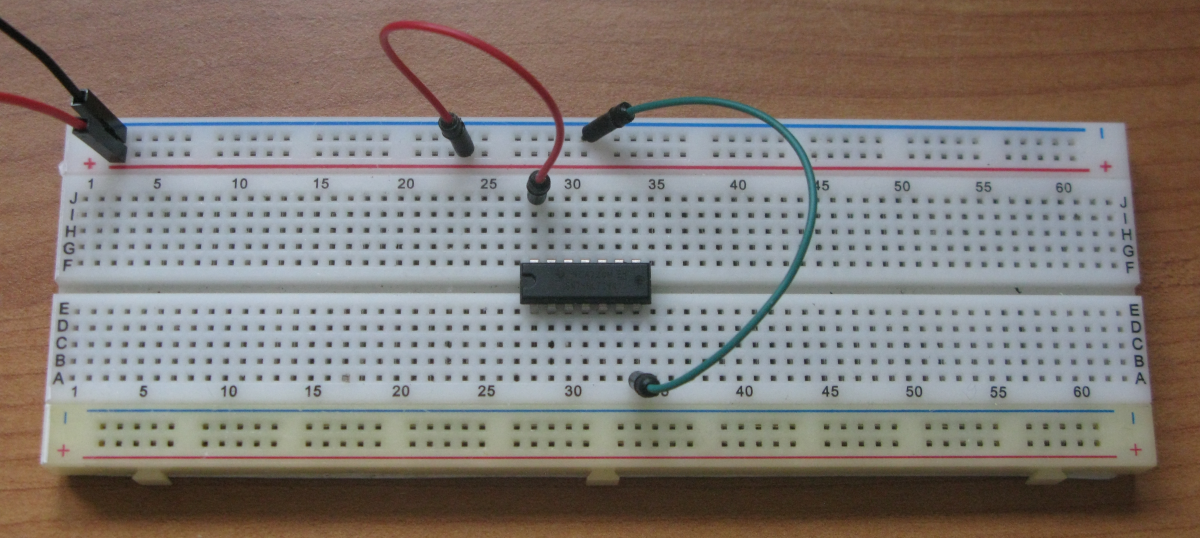
\includegraphics[width=0.9\textwidth]{dip_ic.png}\\
  Tak umieszczamy układy scalone w płytce stykowej. Po lewej stronie widać półokrągle wcięcie na obudowie. Pin 1 jest po lewej na dole.
\end{center}

Na brzegach płytki najczęściej znajdują się podłużne listwy, w których znajdują się grupy takich samych otworków jak
na płytce, pogrupowanych w grupy 2 x 5. Niektóre płytki posiadają też nadrukowane kreski oraz znaki + i -. Te listwy
służą do doprowadzania zasilania do układu na płytce. Otworki w jednej linii wzdłuż płytki są połączone elektrycznie - tworzą tzw.
szynę zasilania. Napięcia zasilania (+ oraz -) z przetwornicy należy podłączać zgodnie z ew. nadrukami na płytce. Zmniejsza to ryzyko
kosztownej pomyłki.
\\

W niektórych płytkach para szyn jest rozdzielona w połowie, i należy o tym pamiętać, ponieważ nie ma na to reguły.
Możesz sprawdzić czy Twoja płytka ma rozdzielone szyny za pomocą multimetru (w trybie omomierza lub testu przewodnictwa). Pozwoli to uniknąć
niespodzianek przy prototypowaniu.

\begin{ProTip}{\normalfont{\strong{Uwaga}}}
  Przed wprowadzaniem jakichkolwiek zmian na płytce stykowej odłącz zasilanie
\end{ProTip}

\begin{Zadanie}{}{}
Za pomocą funkcji testu połączeń swojego miernika, sprawdź, czy Twoja płytka stykowa ma rozdzielone szyny zasilania.
\end{Zadanie}



\section{Układy scalone}
Układy scalone pozwalają szybko i sprawnie konstruować skomplikowane układy elektroniczne przy minimum nakłądu i kosztu. Dzięki nim możemy
używać gotowych bloków cyfrowych (np. licznik, sumator, bramka logiczna) oraz analogowych (regulator napięcia, wzmacniacz operacyjny,
przełączniki anlogowe itp.) zamiast musieć budować je od postaw z elementów elektronicznych. Produkowane są układy o bardzo różnych stopniach
integracji - od bardzo niskich, takich jak np. bramki logiczne, do bardzo wysokich, jak np. gotowe komputery (tzw. SoC - system on a chip).
\\

Na razie skupimy się na prostszych układach - a dokładniej na ich obudowie.

Każdy układ w obudowie DIP ma oznaczony pin nr. 1. Z reguły to oznaczenie ma formę wklęsłego półokręgo na jednym z końców układu albo
okrągłego znaczka przy jednym z pinów na narożniku. W przypadku tego drugiego, pin przy którym znajduje się to oznaczenie to pin nr 1.
W przypadku oznaczonego końca układu, jeżeli obrócisz układ tak aby oznaczenie było na górze, pin nr 1 to lewy górny. W obu przypadkach kolejne piny
liczy się idąc przeciwnie do ruchu wskazówek zegara. Przedstawia to poniższy rysunek:

\textit{jakis schemat obudowy z ponumerowanymi pinami}

Przy podłączaniu układu scalonego ważne jest aby nie pomylić numerów pinów (nóżek). Każdy z nich ma z góry określoną funkcję.



\section{Przygotowanie mikronotrolera}
\textit{tutaj opisać co i jak polutować. Obrazki?}
\begin{ProTip}{\normalfont{\strong{Ostrożnie}}}
  Bardzo możliwe, że Twój mikrokontroler nie będzie miał przylutowanych pinów do połączenia z płytką stykową.
  W takim wypdaku będziesz musiał/musiała użyć lutownicy aby je przylutować.\\
  Podczas pracy, grot (metalowa końcówka) lutownicy jest rozgrzany do 200-400 stopni Celsjusza. Zachowaj ostrożność
  podczas jej używania. Zapamiętaj:
  \begin{itemize}
  \item Zawsze odkładaj lutownicę do stojaka. Nigdy nie kładź jej luzem na stole.
  \item Nigdy nie łap za metalowy koniec lutownicy.
  \item Nie wolno łapać spadającej lutownicy. Nie martw się, zawszę można kupić nową
  \item Grot lutownicy jest gorący przez jakiś czas po wyłączeniu
  \item Nie zostawiaj włączonej lutownicy bez opieki
  \item Przed lutowaniem musisz odłączyć układ od zasilania
  \end{itemize}
\end{ProTip}

Jeżeli Twój mikrokontroler nie ma przylutowanych pinów, musisz przylutować je samemu. Przymierz i odetnij
obcążkami dwa odcinki listwy kołkowej pasujące do otworów na brzegach płytki mikrokontrolera. Włóż piny do otworków
na płytce. następnie odwiń lub wyciągnij odcinek cyny ze szpulki. Włącz lutownicę i odłóż ją na stojak. Jeżeli twoja lutownica
ma ustawienie temperatury, ustaw je na około 250-300 st. C. Daj jej około minuty na osiągnięcie temperatury. Pamiętaj, że grot
lutownicy jest bardzo gorący. Lutownicę należy trzymać tylko i wyłącznie za rękojeść.
\\

Aby zalutować pin w otworze, najpierw dotknij grotem lutownicy
miejsca, które będziesz lutować. Po około sekundzie, dotknij pinu końcówką odcinka cyny.
\\

Postaraj się aby listwy kołkowe były prostopadle do płytki. Jeżeli masz odcinek damskiej listwy, możesz za jego pomocą
umiejscowić piny które lutujesz. Możesz też użyć do tego płytki stykowej. Lutowanie zacznij od czterech pinów na rogach płytki.


\subsection{Instalacja i przygotowanie narzędzi}

Do programowania STM32 potrzebne jest kilka narzędzi

\begin{itemize}
  \item Toolchain arm-none-eabi (\Verb$gcc-arm-none-eabi$) oraz (\Verb$binutils-arm-none-eabi$)
  \item Implementację libC (\Verb$libstdc++-arm-none-eabi-newlib$)
  \item Narzędzie do programowania przez UART (\Verb$stm32flash$)
  \item Bibliotekę \Verb$libopencm3$
\end{itemize}
Wszystkie oprócz ostatniego dostępne są w repozytoriach Debiana (i systemów na nim opartych). Możesz je zainstalować
za pomocą polecenia

\begin{CodeFrame*}[bash]{}
sudo apt install gcc-arm-none-eabi binutils-arm-none-eabi libstdc++-arm-none-eabi stm32flash
\end{CodeFrame*}

Instalacja i kompilacja \Verb$libopencm3$ odbywa się w następujący sposób:

\begin{CodeFrame*}[bash]{}
git clone https://github.com/libopencm3/libopencm3.git
cd libopencm3
make
\end{CodeFrame*}

\subsection{Połączenie mikronotrolera}
\textit {tutaj warto by powrzucać zdjęcia lub rysunki}

\begin{ProTip}{\normalfont{\strong{Uwaga}}}
  Przed podłączaniem lub dokonywaniem jakichkolwiek zmian w układzie, odłącz go od zasilania. Unikniesz
  w ten sposób ryzyka zwarcia i uszkodzenia elementów.
\end{ProTip}

Aby zaprogramować mikrokontroler musisz podłączyć go do przejściówki USB-UART. Umieść płytkę ``okrakiem'' nad przerwą
w płytce stykowej. Za pomocą pasujących kabelków podłącz następujące piny przejściówki (nie podłączaj jeszcze
przejściówki do komputera) do pinów na mikrokontrolerze:
\begin{itemize}
\item masę (GND) do (dowolnej) masy miktrokontrolera (GND lub G)
\item RX do TX mikrokontrolera (pin A9)
\item TX do RX mikrokontrolera (pin A10)
\item 5V do 5V mikrokontrolera
\end{itemize}

Za pomocą obcążków lub pęsety przełóż górną (patrząc na mikrokontroler tak aby port USB był po lewej) zworkę na
pozycję ``1''.

Sprawdź wszystkie połączenia i podłącz przejściówkę do portu USB komputera. Na mikrokontrolerze powinna zaświecić się tylko czerwona dioda
\textit{PWR}

Możesz sprawdzić połączenie z mikrokontrolerem używając \Verb$stm32flash$ do obliczenia sumy kontrolnej pamięci mikrokontrolera.
Jeżeli polecenie poniżej nie zgłosi błędów, wszystko działa poprawnie.

\begin{CodeFrame*}[bash]{}
stm32flash -C /dev/ttyUSB0
\end{CodeFrame*}

Tak przygotowany mikrokontroler jest gotowy do pracy.








\end{document}
